\documentclass[12pt, a4paper]{report}

\usepackage[margin=1in]{geometry}
\usepackage[utf8]{inputenc}
\usepackage[T1]{fontenc}

\usepackage{times}

\usepackage{float}

\usepackage{url}
\usepackage{xurl} % Avoids URLs to overfull \hbox

\usepackage{graphicx}
\graphicspath{{img/}} % global configuration
\usepackage[colorlinks=false, pdfborder={0 0 0}]{hyperref}

\usepackage{tabularray}

\usepackage{listings}
\usepackage[table, svgnames]{xcolor}

\title{
  Data Compression
}
\author{
  Enrico Marchionni\\
  \texttt{enrico.marchionni@studio.unibo.it}
}
\date{\today}

% Package to keep track of the total number of pages
\usepackage{lastpage}
\usepackage{fancyhdr}

\fancypagestyle{fancy}{
  \fancyhf{}
  \fancyfoot[C]{\thepage\ of \pageref{LastPage}}
  \renewcommand{\headrulewidth}{0pt}
  \renewcommand{\footrulewidth}{0.4pt}
}

\fancypagestyle{plain}{
  \fancyhf{}
  \fancyfoot[C]{\thepage\ of \pageref{LastPage}}
  \renewcommand{\headrulewidth}{0pt}
  \renewcommand{\footrulewidth}{0.4pt}
}

\pagestyle{fancy}

\usepackage[backend=biber, style=alphabetic, sorting=ydnt]{biblatex}
\addbibresource{references.bib}

\usepackage{amsthm} % to make definitions
\newtheorem{definition}{Definition}[section] % custom environment for definitions
\newtheorem{example}{Example}

% for graphs and overlaying text
\usepackage{tikz}
\usepackage{pgfplots}
\pgfplotsset{compat=1.18}
\usepackage{amsmath} % For math symbols

\begin{document}

\maketitle

\begin{abstract}

Data compression is intended as the practice of reducing the size of binary digital data.
It could be considered as a procedure that takes a bit-stream in input and returns another bit-stream as output.
The output stream may be of equal length or shorter than the input.

The key to understand data compression is to discuss the distinction between data and information.
It can be said that data is how information is represented\footnote{ex. the number 0 can be expressed in binary as a sequence of a
certain number of zeros, from \(1\) to \(\infty\), and we know that calculators use at least 8 bits, let's say \(n\)
(considering it as a multiple of 8), to represent an integer number. So at the end \(n - 1\) bits are redundant in the 0
representation on a calculator.}. In simple terms, data can be compressed because its original representation is not the shortest
possible. The goal of data compression is to reduce data by maintaining the same information.

The counterpart is that in our time data is intrinsically redundant. And this redundancy is needed.
So data compression isn't only a procedure that goes from a bit-stream to another one not longer, but it requires also another
procedure that regenerates the original bit-stream of data, necessary for practical use, from the previously given output
bit-stream of information.

\dots % difference between information and meaning???

\end{abstract}

\tableofcontents

\chapter{Information Theory}

In 1948, Shannon\footnote{Claude Elwood Shannon (1916–2001) was an American mathematician, electrical engineer, computer
scientist, cryptographer and inventor known as the "father of information theory".}, while working at the Bell Telephone
Laboratories, published "A Mathematical Theory of Communication" \cite{AMathematicalTheoryOfCommunication}, a seminal paper that
marked the birth of information theory. In that paper, Shannon defined the concept of "information" and proposed a precise way to
quantify it-in his theory, the fundamental unit of information is the bit.

Moreover, this discipline plays behind the concepts of entropy, randomness and data compression, all topics that will be discussed
later on.

\section{Quantifying Information}

For what concerns data compression, information of theory has developed a usable measure of the information we get from observing
the occurrence of an event having probability \(p\). Therefore information is defined in terms of the probability.

The information measure \(I(p)\) has to match the following axioms (from \cite{AnIntroductionToInformationTheoryAndEntropy}):

\begin{itemize}
  \item Information is non negative: \(I(p) \geq 0\).
  \item If an event has probability 1, we get no information: \(I(1) = 0\).
  \item If two independent events occur (whose probability is the product of their individual probabilities), then the information
  we get from observing the events is the sum of the two computed individually: \(I(p_1 \cdot p_2) = I(p_1) + I(p_2)\).
  \item Information measure must be continuous and monotonic (slight changes in probability should result in slight changes in
  information).
\end{itemize}

Considering the previous properties as axioms it can be said that: \(I(p^2) = I(p \cdot p) = I(p) + I(p) = 2 \cdot I(p)\).
Thus: \(I(p^n) = n \cdot I(p)\) (by induction).
Then: \(I(p) = I(p^{(\frac{1}{m})^m}) = m \cdot I(p^{\frac{1}{m}})\), so \(I(p^{\frac{1}{m}}) = \frac{1}{m} \cdot I(P)\),
therefore: \(I(p^{\frac{n}{m}}) = \frac{n}{m} \cdot I(p)\).
In general, considering \(r\) as a real number: \(I(p^a) = a \cdot I(p)\).

From this analysis it was discovered that:

\begin{equation} \label{eq:information1}
  I(p) = - \log_b p \ (= \log_b \frac{1}{p})
\end{equation}

Where: \(p = b_1^{\log_{b_1} p}\) and therefore: \(\log_{b_2} p = \log_{b_2} b_1^{\log_{b_1} p} = \log_{b_2} b_1 \cdot \log_{b_1}
p\). So: \(\log_{b_2} b_1\) is a constant, a scaling factor.
From another point of view it is a simple change in the unit of measurement.

For this reason:

\begin{equation} \label{eq:information2}
  I(p) = - \log_2 p
\end{equation}

\autoref{eq:information2} is the same expression of \autoref{eq:information1} where the unit of measurement is called bits
(look at \autoref{tab:information_units}). \autoref{eq:information1} was first introduced by Hartley\footnote{Ralph Vinton Lyon
Hartley (1888-1970) was an American electronics researcher. He invented the Hartley oscillator and the Hartley transform,
and contributed to the foundations of information theory.} in 1928 trying to measure uncertainty, without talking about
probability, and lately reviewed by Shannon.

\begin{table}[H]
  \begin{tblr}{
      colspec={X[l]X[l]},
      width=\textwidth,
      row{odd}={gray!15},
      row{even}={white},
      row{1}={bg=gray!90,fg=white},
      colsep=4pt
    }
      \textbf{Unit of measurement} & \textbf{Base} \\
      bit (or shannon) & \(2\) \\
      \hline
      trit & \(3\) \\
      \hline
      nat (natural unit of information) & \(e\) \\
      \hline
      hartley (or dit) & \(10\) \\
      \hline
  \end{tblr}
  \caption{\label{tab:information_units} Information units of measurement}
\end{table}

\begin{example}
Let's talk about flipping a fair coin n times. It gives us: \(- \log_2 \frac{1}{2}^n = \log_2 2^n = n \cdot \log_2 2 = n\) bits of
information. In fact a sequence of heads (coded as \(1\)) and tails (coded as \(0\)) could be expressed as: \(010010111\dots\),
these are the \(n\) bits of information.
\end{example}

\chapter{Entropy}

% DEFINITION
% \begin{definition}
% \textbf{Entropy}\footnote{\url{https://dictionary.cambridge.org/dictionary/english/entropy}} is the amount of order or lack of
% order in a system.
% \end{definition}

Entropy is a concept that was explained in many fields. Previously defined by Clausius\footnote{Rudolf Julius Emanuel Clausius
(1822–1888) was a German physicist and mathematician and is considered one of the central founding fathers of the science of
thermodynamics.} and Boltzmann\footnote{Ludwig Eduard Boltzmann (1844–1906) was an Austrian physicist and philosopher. His
greatest achievements were the development of statistical mechanics and the statistical explanation of the second law of
thermodynamics.} was later used by Shannon. It is believed that these three definitions are indeed equivalent although no formal
proof of this is available (as discussed in \cite{EntropyAndInformationTheoryUsesAndMisuses}).

\section{Quantifying Entropy}

Here is how Shannon introduced the measure of Information:
\begin{quote}
Suppose we have a set of possible events whose probabilities of occurrence are \(p_1, p_2, \dots, p_n\). These probabilities are
known but that is all we know concerning which event will occur. Can we find a measure of how much "choice" is involved in the
selection of the event or how uncertain we are of the outcome?
\end{quote}
If there is such a measure, say, \(H(p_1, p_2, \dots, p_n)\)\footnote{Where \(H\) refers to Hartley.}, it is reasonable to require
of it the following properties:
\begin{itemize}
  \item \(H\) should be continuous in the \(p_i\).
  \item If all the \(p_i\) are equal, \(p_i = \frac{1}{n}\) then \(H\) should be a monotonic increasing function of \(n\). With
  equally likely events there is more choice, or uncertainty, when there are more possible events.
  \item If a choice be broken down into two successive choices, the original \(H\) should be the weighted sum of the individual
  values of \(H\).
\end{itemize}

Then Shannon proved that the only \(H\) satisfying the three assumptions above has the form:

\begin{equation} \label{eq:entropy1}
  H = -K \sum_{i = 1}^{n} p_i \ln p_i
\end{equation}

\autoref{eq:entropy1} includes a constant \(K\), in the Shannon article it is any constant. In application to thermodynamics \(K\)
turns into Boltzmann Constant. It is simply a scaling factor. Note that if \(K\) is \(\frac{1}{\ln b}\) or equivalently
\(\log_b e\), the formula, considering only \(K\) and the logarithm, becomes \(\log_b e \cdot \ln p\) that is the same of
\(\log_b e^{\ln p}\) that can be simply written as \(\log_b p\).

So \(H\) can be simply reformulated as:

\begin{equation} \label{eq:entropy2}
  H(P) = - \sum_{i = 1}^{n} p_i \log_2 p_i
\end{equation}

Where \(P = {p_1, p_2, \dots, p_n}\) is the distribution of probability considered.
remind that in \autoref{eq:entropy2} base \(2\) could be a general base \(b\) and it can be simply view as a simple change in the
unit of measurement (as it was seen in \autoref{tab:information_units}).

An intuitive way to explain the origin of this formula is now discussed. We want to obtain the average amount of information from
each symbol we see in a stream. Let's suppose we start from \(n\) symbols \(a_1, a_1, \dots, a_n\).
A stream of these symbols is provided with probabilities \(p_1, p_1, \dots, p_n\) respectively.
As it was seen in \autoref{eq:information2} for a symbol \(a_i\) we get \(-\log_2 p_i\) information.
In a long run, say \(N\) observations, we will see (approximately) \(N \cdot p_i\) occurrences of the symbol \(a_i\).
Thus in the \(N\) independent observations, we will get total information of:

\begin{equation} \label{eq:information_entropy1}
  I = - \sum_{i = 1}^n (N \cdot p_i) \log_2 p_i
\end{equation}

So then, from \autoref{eq:information_entropy1} the average information is:

\begin{equation} \label{eq:information_entropy2}
  \frac{I}{N} = - \frac{1}{N} \sum_{i = 1}^n (N \cdot p_i) \log_2 p_i = - \sum_{i = 1}^n p_i \log_2 p_i
\end{equation}

At this point we get \autoref{eq:information_entropy2} that is the same as \autoref{eq:entropy2}.
Furthermore, it is shown in \autoref{eq:entropy_bounds} that \(H(P)\) is bounded (for further information see
\cite{AnIntroductionToInformationTheoryAndEntropy}):

\begin{equation} \label{eq:entropy_bounds}
  0 \leq H(P) \leq \log_2 n
\end{equation}

\begin{example}
Returning to the example of the coin, in \autoref{fig:entropy_graph} it is shown an example of the entropy in function of the
probability of heads or tails when flipping a fair coin.

\begin{figure}[H]
  \centering
    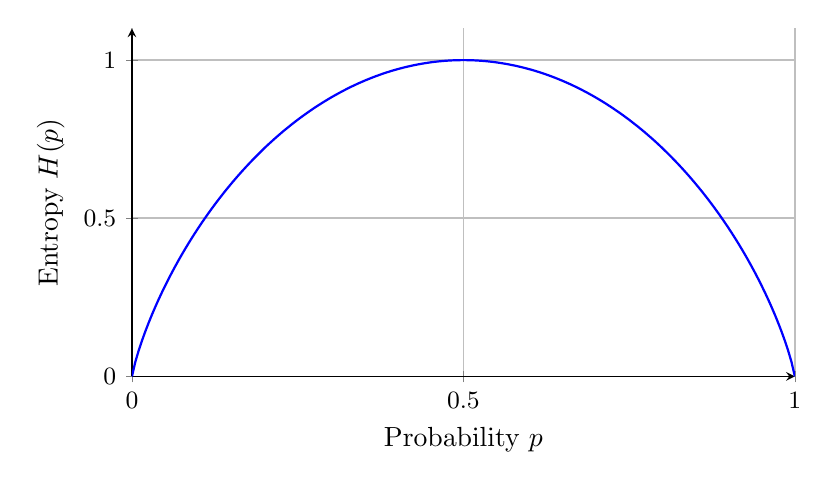
\begin{tikzpicture}
        \begin{axis}[
            width=10cm,
            height=6cm,
            xlabel={Probability \( p \)},
            ylabel={Entropy \( H(p) \)},
            ymin=0, ymax=1.1,
            xmin=0, xmax=1,
            ytick={0, 0.5, 1},
            xtick={0, 0.5, 1},
            domain=0:1,
            samples=200,
            grid=both,
            major grid style={line width=0.6pt, draw=gray!50},
            minor grid style={line width=0.3pt, draw=gray!30},
            tick label style={font=\small},
            axis lines=left
        ]
            \addplot[
                thick,
                blue,
            ]
            {-x*log2(x) - (1-x)*log2(1-x)} node[pos=0.5, above, sloped, xshift=-0.5cm, yshift=0.3cm] {};
        \end{axis}
    \end{tikzpicture}
    \caption{\label{fig:entropy_graph} Graph of entropy \( H(p) = -p \log_2(p) - (1-p) \log_2(1-p) \) for a fair coin toss.}
\end{figure}
\end{example}

\chapter{Randomness}

Compression, logically, can be interpreted as the removal of redundancy. The compressed data therefore has no structure and cannot
be distinguished from random data; in fact, it is random (\cite{AConciseIntroductionToDataCompression}).

\section{Kolmogorov}

% Kolmogorov complexity

\begin{definition}
\textbf{Kolmogorov complexity} of a binary sequence is the length of the shortest binary program that generates that sequence on a
universal Turing machine (\cite{ThreeApproachesToTheQuantitativeDefinitionOfInformation}).
\end{definition}

The concept essentially asserts that a binary sequence is considered random if there is no algorithm shorter than the sequence
itself that can generate it.

That is related to the concept of incompressibility in algorithmic randomness: a random sequence cannot be compressed into a
shorter representation than its original size.

So, loosely speaking, the randomness (or Kolmogorov complexity) of a finite sequence is equal to its shortest description.

It is known that the Kolmogorov complexity is not computable.

\section{Martin-Lof} % andrebbero messi 2 punti sopra alla o

Martin-Lof in Algorithmic Randomness and Complexity (\cite{TheDefinitionOfRandomSequences}) shows that the random elements as
defined by Kolmogorov possess all conceivable statistical properties of randomness.

He also extended the definition for random elements with three approaches to the definition of algorithmic randomness for infinite
sequences:

\begin{definition}
The \textbf{computational paradigm}: Random sequences are those whose initial segments are all hard  to describe, or,
equivalently, hard to compress.
\end{definition}

\begin{definition}
The \textbf{measure-theoretic paradigm}: Random sequences  are those with no "effectively rare" properties. If the class of
sequences satisfying a given property is an effectively null set, then a random sequence should not have this property.
This approach is the same as the stochastic paradigm: a random sequence should pass all effective statistical tests.
\end{definition}

\begin{definition}
The \textbf{unpredictability paradigm}: This approach stems from what is probably the most intuitive conception of randomness,
namely that one should not be able to predict the next bit of a random sequence, even if one knows all preceding bits, in the same
way that a coin toss is unpredictable even given the results of previous coin tosses.
\end{definition}

Taken from \cite{AlgorithmicRandomnessAndComplexity}.

The previous citations aim to observe that the idea of Kolmogorov that random generators didn't exist was lately reviewed and
while remaining true, extended to infinite sequences.

\section{Random Sequences}

A random sequence should satisfy three conditions:

\begin{itemize}
  \item The sequence follows a uniform distribution.
  \item Each element of the sequence is independent of each other.
  \item The rest of the sequence can not be predicted from any sequence.
\end{itemize}

Random numbers can be divided into two categories: true random numbers and pseudo-random numbers.
True random number generators (RNGs) are composed of two parts: entropy source and algorithm post-processing.
Pseudo random number generators (PRNGs) take a seed as input and generate an output sequence by function.

\appendix

\printbibliography

\end{document}
